\section{Auswertung}
\label{sec:Autswertung}
\subsection{Wheatston’sche Messbrücke}
Die Wheatonsche Brückenschaltung weist im Verhältnis der Widerstände $R_3$ und $R_4$ 
einen systematischen Fehler von $\increment=0.005\cdot\sfrac{R_3}{R_4}$ auf. Für die erste
Messung wird der Widerstand mit dem Theoriewert $10=\qty{239}{\ohm}$ genutzt, welcher dann experimentell
bestimmt wurde. Mit den Messdaten aus Tab. \ref{tab:Auswertung_1}, sowie über die Abgleichbedingung \eqref{eq:Abgleichbed} und die Gaußsche Fehlerfortplflanzung
ergibt sich
\begin{equation*}
    R_\text{x}=\qty{271+-1.4}{\ohm}\,.
\end{equation*}
Die Gaußsche Fehlerfortplflanzung wurde nach der Formel 
\begin{equation*}
    \increment f=\sqrt{\sum_{k=1}^{n}\biggl(\frac{\partial f}{\partial x_\text{k}}\biggr)^2(\increment x_\text{k})^2}
    \label{eq:gauss}
\end{equation*}
mittels Python durchgeführt. Dabei ist $f$ die zur Berechnung der Größe gegebene Formel 
und $x_k$ dessen Argumente. $\increment x_k$ ist der jeweilige Fehler der einzelnen Argumente.
Damit ergibt sich für die erste Messung eine Abweichung von 13.5\% gegenüber dem Theoriewert.\\ \noindent
Die zweite Messung wird mit Wert 12 als Unbekannte durchgeführt, die Messdaten sind in Tab. \ref{tab:Auswertung_1} dargestellt.
Es ergibt sich folgender Wert
\begin{equation*}
    R_\text{x}=\qty{322+-1.6}{\ohm}\,.
\end{equation*}
Gegenüber dem Theoriewert von $\qty{390.4}{\ohm}$ ist dies eine Abweichung von $17,4\%$.
\begin{table}[H]
    \centering
    \caption{Verwendete Widerstände für die Wheatonschen Brückenschaltung.}
    \label{tab:Auswertung_1}
    \begin{tblr}{colspec={c| c c c }}
        \toprule
        Messung & $R_2$ / $\Omega$ & $R_3$ / $\Omega$ & $R_4$ / $\Omega$ \\  
        \midrule
        1 & 664 & 290 & 710\\
        2 & 664 & 327 & 673\\
        \bottomrule
    \end{tblr}
\end{table}
\subsection{Kapatitätsmessbruecke}
Mithilfe der Kapatitätsmessbruecke werden pro Messung ein Widerstand, mittels
\eqref{eq:Abgleichbed}, und ein kapazitiver Widerstand, mittels \eqref{eq:kapawiderstand},
bestimmt.
Zur ersten Messung werden $R$ (Wert 12) und $C$ (Wert 1) mit den Werten aus Tab. \ref{tab:Auswertung_2} zu
\begin{align*} 
R_\text{x}&=\qty{393+-2}{\ohm} \text{ und}\\
C_\text{x}&=\qty{673.6+-3.4}{\nano\farad} 
\end{align*} bestimmt. 
Da sich auch $C_x$ über das Verhältnis $\sfrac{R_3}{R_4}$ bestimmen lässt, gilt der 
gleiche relative Fehler. Für $R$ ergibt sich eine Abweichung von $0,7\%$, von dem Theoriewert von $\qty{390.4}{\ohm}$.
Für $C$ ergibt sich eine Abweichung von $2,1\%$, von dem Theoriewert von $\qty{660}{\nano\farad}$.
Zur zweiten Messreihe ist $C$ gegeben durch $2 \, \cdot$ Wert 3, $R$ bleibt unverändert mit Wert 12.
Mit den verwendeten Wiederständen und Kondensatoren aus Tab. \ref{tab:Auswertung_2} ergeben sich folgende Werte
\begin{align*}
    R_x&=\qty{370+-1.9}{\ohm}\,\\
    C_x&=\qty{716+-4}{\nano\farad}\,.
\end{align*}
Die Fehler zu den Theoriewerten $\qty{390.4}{\ohm}$ und $\qty{839.89}{\nano\farad}$ betragen
\begin{align*}
    \increment{R_x}&=5,2\%\,\\
    \increment{C_x}&=14,8\%\,.
\end{align*}
\begin{table}
    \centering
    \caption{Verwendete Widerstände und Kondensatoren für die Kapatitätsmessbrücke.}
    \label{tab:Auswertung_2}
    \begin{tblr}{colspec={c| c c c c}}
        \toprule
        Messung & $C_2$ / nF & $R_2$ / $\Omega$ & $R_3$ / $\Omega$ & $R_4$ / $\Omega$ \\
    \midrule
    1 & 399 & 664 & 372 & 628 \\
    2 & 399 & 664 & 358 & 642 \\
    \bottomrule
    \end{tblr}
\end{table}
\subsection{Induktivitätsmessbruecke}
Um die Induktivität einer Spule zu bestimmen wird die, in Abb.
\ref{fig:Induktivitaetsmessbruecke},
dargestellte Induktivitätsmessbrücke verwendet.
Die Induktivität berechnet sich dann nach Gleichung \eqref{eq:induktivität}.
$R$ und $L$ sind zusammengefasst zu Wert 19, für welchen die Theoriewerte $\qty{108.7}{\ohm}$ und $\qty{26.96}{\milli\henry}$
angegeben sind.
Aus den verwendeten Widerständen und der verwendeten Induktivität, welche in Tab. \ref{tab:Auswertung_3}
dargestellt sind, ergeben sich folgende Werte
\begin{align*}
    R_x&=\qty{156.8+-0.8}{\ohm}\,\\
    L_x&=\qty{6.5+-0.03}{\henry}\,.
\end{align*}
Die Fehler ergeben sich zu $44,2\%$ für den Widerstand und $75,9\%$ für die Induktivität.
\begin{table}
    \centering
    \caption{Verwendete Widerstände und Induktivitäten für die Induktivitätsmessbrücke.}
    \label{tab:Auswertung_3}
    \begin{tblr}{colspec={c | c c c c}}
        \toprule
        Messung & $L_2$ / H & $R_2$ / $\Omega$ & $R_3$ / $\Omega$ & $R_4$ / $\Omega$ \\
    \midrule
    1 & 27,5 & 664 & 191 & 809\\
    \bottomrule
    \end{tblr}
\end{table}
\subsection{Maxwell-Brücke}
Die Maxwell-Brücke ist die zweite durchgeführte Methode zur Bestimmung der Induktivität.
Die unbekannten Werte werden gleich gelassen (Wert 19), jedoch hat sich das Schaltbild geändert.
Es ergeben sich mittels Gleichung \eqref{eq:maxwell} und den verwendeten Widerständen und Kondesatoren
aus Tab. \ref{tab:Auswertung_4} die Werte
\begin{align*}
    R_x&=\qty{62+-2.6}{\ohm}\\ \,
    L_x&=\qty{9.8+-0.3}{\milli\henry}\,.
\end{align*}
Die Fehler belaufen sich auf eine Induktivitätsabweichung von $100\%$ und eine 
Widerstandsabweichung von $42.8\%$\, gegenüber den Theoriewerten $\qty{108.7}{\ohm}$ und $\qty{26.96}{\milli\henry}$.
\begin{table}
    \centering
    \caption{Verwendete Widerstände und Kondensatoren für die Maxwell-Brücke.}
    \label{tab:Auswertung_4}
    \begin{tblr}{colspec={c|c c c c}}
        \toprule
        Messung & $C_4$ / nF & $R_2$ / $\Omega$ & $R_3$ / $\Omega$ & $R_4$ / $\Omega$ \\
        \midrule
        1 & 399 & 664 & 37 & 395\\
        \bottomrule
    \end{tblr}
\end{table}
\subsection{Wien-Robinson-Brücke}
In diesem Teil des Versuches wird die Frequenz nicht mehr konstant eingestellt, sondern
modulliert. Es soll die Frequenzabhängigkeit der Spannung gemessen werden. Dabei werden,
die in Tabelle \ref{tab:wien-robinson} aufgeführten, Daten messen.
\begin{table}
    \centering
    \label{tab:wien-robinson}
    \caption{Spannung in Abhängigkeit der Frequenz zur Wien-Robinson-Brücken-Schaltung.}
    \begin{tblr}{colspec={c c||c c}}
    \toprule
    $\nu$ / Hz & $U$ / mV & $\nu$ / Hz & $U$ / mV \\
    \midrule
    50   & 144.0& 1000 & 156\\
    100  & 96.0 & 1500 & 160\\
    150  & 62.0 & 2000 & 160\\
    200  & 21.8 & 2500 & 160\\
    250  & 6.6  & 3000 & 160\\
    300  & 26.0 & 3500 & 160\\
    350  & 44.8 & 4000 & 160\\
    400  & 58.4 & 4500 & 160\\
    450  & 77.6 & 5000 & 160\\
    500  & 79.2\\
\bottomrule    
\end{tblr}
\end{table}
Die Theoriekurve, auf der die Messwerte im Idealfall liegen sollten, ist beschrieben
durch Gleichung \eqref{eq:theoriekurve}\,.
Da die Spannung in verschiedenen Schritten gemessen wird, wird die $x$-Skala
logarithmiert. Dabei werden folgende Werte verwendet
\begin{align*}
    R'&=\qty{332}{\ohm}\,\\
    2R'&=\qty{664}{\ohm}\,\\
    C&=\qty{994}{\nano\farad}\,\\
    R&=\qty{664}{\ohm}\,\\
    U_\text{S}&=\qty{0.5}{\volt}\,.
\end{align*}
Die nach Gleichung \eqref{eq:theoriekurve} aufgetragenen Messwerte, sowie die
Theoriekurve sind in Abb. \ref{fig:plot} visualisiert.
\begin{figure}
    \centering
    \label{fig:plot}
    \caption{Die Spannung aufgetragen gegen den Logarithmus der Frqeuenz.}
    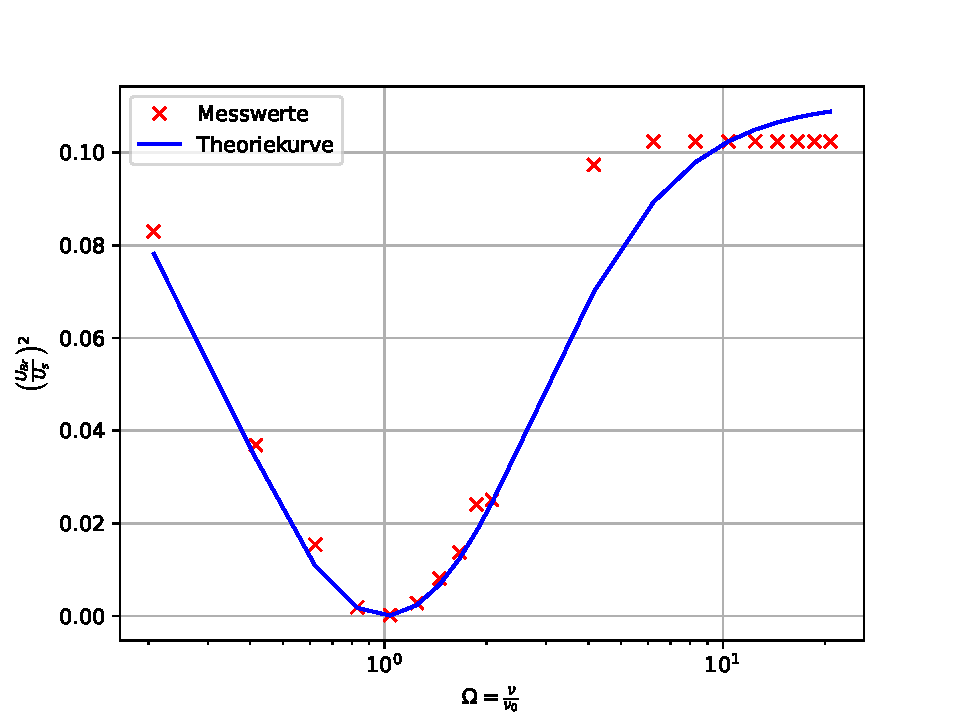
\includegraphics[width=\textwidth]{python/fit.pdf}
\end{figure}
